\documentclass[12pt]{article}
\usepackage{amsmath}
\usepackage{amsthm}
\usepackage{amssymb}
\usepackage{enumerate}
\usepackage{graphicx}
%\usepackage{fullpage}
\usepackage[top=1in, bottom=1in, left=0.8in, right=1in]{geometry}
\usepackage{multicol}
\usepackage{algpseudocode} 
\usepackage{algorithm}
\usepackage{float}
\usepackage{wrapfig}
\usepackage{units}
\usepackage{setspace}
\usepackage{placeins}
\doublespacing

\setlength{\columnsep}{0.1pc}

\title{Ropes - Alternative String Representation}
\author{Leo Martel, Paul Martinez, Andy Moreland}
\date{\today}
\begin{document}

\maketitle
\vspace{-0.3in}
\rule{\linewidth}{0.4pt}

%%%%%%%%%%%%%%%%%%%%%%%%%%%%%%%%%%%%%%%%%%%

\section{Introduction}

In this paper we will discuss the Rope data structure, a data structure intended to serve as a more robust and more performant alternative to the traditional String type offered in most languages.
The seminal paper regarding Ropes was written by Hans-J. Boehm, Russ Atkinson and Michael Plass in 1995.
We will provide an overview of their paper, beginning with their justification for Ropes in the first place.
We will continue with a more technical exploration of the implementation details and running time guarantees of the various operations that Ropes support.
Finally, we will conclude with an overview of our contributions. In particular, we have implemented our own Rope in $C++$ and we provide benchmarks that demonstrate its performance. We have also implemented a $D3$\footnote{http://d3js.org/} based visualization which helps demonstrate the internal workings of a rope. We briefly discuss this implementation before we conclude.

\section{Justification for Expanded String Type}

Historically languages like C and Pascal have implemented strings essentially as arrays of characters. Generally this array is of fixed length and basic operations can be implemented in terms of standard array access. Higher level operations are usually provided in the form of library functions: C, for example, provides substring, concatenation and length operations. Many languages implement the string type in the most bare-bones way possible: C, for example, does not even include length alongside the character data.

Boehm, Russ and Plass (BAP) begin their paper by discussing the problems that follow from this type of approach. They suggest the Rope datastructure and demonstrate that it improves on many of these flaws. We will summarize their ideas here.

BAP believe that one of the biggest problems with traditional arrays is the fact that they are mutable. Robust system design dictates that we separate our systems into a collection of modules which interact over tightly-guarded interfaces. Unfortunately, for the sake of efficiency strings are often passed through these interfaces by reference. This means that the client of a given module must take care not to accidentally modify a string that it receives lest it incidentally change the internal state of the module. This violates the Principle of Encapsulation. Accordingly, BAP have designed the Rope data structure to efficiently support important operations while remaining immutable: the Rope is a copy-on-write structure.

In additional to enabling immutability, BAP's Rope design supports efficient concatenation, substring and deletion operations which do not require excessive space overhead. At the time of writing this was particularly relevant because, as BAP joke, "six-month-old child randomly typing at a workstation would routinely crash some older UNIX kernels due to a buffer size limitation." Even editors which are now considered efficient, like vi, used to struggle with long line lengths. By contrast, the Rope structure scales well to handle large strings.

\section{Implementation and Running Time}

\begin{figure}[t]
\begin{centering}
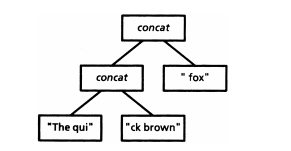
\includegraphics[scale=0.75]{simple_rope}
\caption{This figure demonstrates a potential Rope structure for the string, ``The quick brown fox.'' Notice that the string is broken up over several leaf nodes which are joined by concatenation nodes.}\label{representation}
\end{centering}
\end{figure}

In this section we will discuss the representation of the Rope datastructure as well as the implementaton and running times of various common operations on it.

First, we will develop the representation. As a motivating example, consider the concatenation of two strings. If we want to support immutability naively we might decide to copy both strings into a new buffer. However, this is extremely performance inefficient if the strings are large, and requires making full duplicates of the strings before we have actually modified anything. This suggests that a reasonable approach would be to try to loosely join our target strings together: in particular, we will gradually form a tree structure of joined strings.

More directly: a Rope is a binary tree whose interior nodes are called \emph{concatenation nodes}, since they represent the concatenation of two smaller strings, and whose leaves are \emph{flat} strings which are represented as character arrays. A Rope for a simple string is shown in Figure \ref{representation}. BAP note that because the leaf notes are immutable, a sequence of concatenation and substring calls could lead to many of these nodes being shared among multiple ropes. Technically this would make the Rope a directed acyclic graph rather than a tree, but for the sake of brevity we will refer to the structure as a tree since we will generally be considering only a single rope at a time.

By virtue of this tree structure, alongside a few minor adjustments, our Rope structure is able to efficiently support the following operations, where $n$ is taken to be the length of the string represented by the Rope:

\begin{enumerate}
\item \emph{concat$(r_1, r_2)$}: returns a new rope structure which contains $r_1$ followed by $r_2$ in time $O(1)$
\item \emph{substring(start, len)}: returns a new rope structure consisting of the characters between (inclusive) indices $start$ and $start + end$ in time $O(\log(n)$
\item \emph{charAt(i)}: returns the character stored at index $i$ in time $O(\log(n))$
\item \emph{iteration} over each character more efficiently than by repeated charAt calls in time $O(n)$
\end{enumerate}

These running times all assume a balanced-tree representation. However, BAP argue in the paper that tree-rebalancing operations are very expensive in practice and so should be avoided when possible and defered until a later point. In practice, this may cause some of these asymptotic bounds to slip.

In the following subsections we will describe how each of these operations are implemented and analyze their running time bounds.

\subsection{Concatenation}

Concatenation is one of the most important operations for a Rope. Generally, concatenating two ropes together is simply a matter of creating a new concatenation node and setting the left and right children of it to be the two Ropes to be concatenated. This is trivially a constant time operation. However, BAP suggest a few optimizations to this operation.

The first optimization they sugest is one for the common case of concatenating two short flat ropes (i.e. leaves). If the ropes are determined to be sufficiently short then BAP suggest that the implementor should simply construct a new leaf node which contains the concatenated strings. This cuts down on space overhead since we do not have to store an additional concatenation node and also speeds up future operations.

BAP also suggest an optimization for the slightly more complicated case of appending a flat rope, $r_1$, to a rope whose root's right child is also a flat rope, say $r_2$. In this case we simply produce a new flat rope, $r_3$, which contains the concatenation of $r_1$ and $r_2$. Then, we concatenate $r_3$ to the left child of our original rope. This optimization applies identically in the case of prepending a flat rope to a rope whose root's left child is flat.

Together these two optimizations cause the construction of a rope by repeated small concatenations to be very efficient. If we did not do this then we would often end up with a degenerate left-spine structure which would inflict roughly $O(n)$-time bounds on our aforementioned operations until the tree were rebalanced. Using these optimizations avoids the need for the expensive rebalance operation at all.

The authors also suggest that the concatenation operation hold the logic for rebalancing. If, during a rebalance, the sizes of the left and right subtrees of the new concatenation node are significantly unequal, it would be reasonable to trigger a rebalancing operation to correct this problem. 


\subsection{Substring}


\begin{figure}[t]
\begin{algorithmic}
  \Function{substring}{$concat(r_1, r_2), start, len$}
  \If{$\text{start} \le 0 \text{ and } \text{len} \ge \text{length}(r_1)$}
  \State \Return $r_1$
  \Else
  \State $left \gets substr(r_1, start, len)$
  \EndIf

  \If{$\text{start} \le \text{length}(r_1) \text{ and } \text{start} + \text{len } \ge \text{length}(r_1) + \text{length}(r_2)$}
  \State \Return $r_2$
  \Else
  \State $right \gets substr(r_2, start - \text{length}(r_1), len - \text{length}(left))$
  \EndIf
  \State \Return $concat(left, right)$
  \EndFunction
\end{algorithmic}
\caption{Psuedocode for the substring operation}\label{substring}
\end{figure}


The substring operation on a rope is fairly trivial to implement, but requires us to discuss a few more implementation details of a rope. In particular, in order to efficiently support substrings it is necessary for us to store some metadata in concatenation nodes. So, in addition to the left and right child pointers that we have previously assumed, we will also assume that a concatenation node stores the size of the substring that appears beneath it in the tree. This size metadata can easily be maintained through concatenation operations by simply computing the sum of the size tags in the left and right child pointers if they are concatenation nodes, or by computing the actual string length for leaf nodes. Maintaining this size data through rebalance operations depends on the precise mechanism of rebalancing, but, for instance, is possible to do at no asymptotic overhead if the Rope is stored using a rotation-based balanced tree representation.

Psuedocode for this operation is presented in Figure \ref{substring}. The concept is straightforward: effectively, we recursively execute substring until we find a subrope containing the start of our range. Then, we take as much of that rope as we need and recurse on its sibling node if we have not satisfied the entire substring range. During this time we produce at most two new concatenation nodes: potentially, one for the leftmost and rightmost edges of the substring range.

The running time for this algorithm is clearly bounded by the tree height since it potentially recurses until it hits leaves. If we are diligent about keeping our Rope structure balanced, then it should take $O(\log(n))$ time in order to satisfy the entire request assuming that only a constant number of leaf nodes are required.

BAP also suggest an optimization for this operation. They note that instead of explicitly constructing a new rope in order to satisfy the substring request, it is possible to add a special \emph{substring node} which would represent an unevaluated substring request. This takes advantage of the fact that if no one ever requests the contents of the substring it is actually pointless to do the work of computing it. They call this ``lazy substring computation.'' It is particularly advantageous if we are asked to compute long substrings of ropes that are mostly flat.

\subsection{Indexed Lookup}

Another operation that we want our Rope to support is the \emph{charAt} operation. This is a very simple operation to implement if we make an observation about the structure of our tree. Effectively, although we do not directly store keys for our tree nodes, it is possible to compute them on the fly and perform a regular binary search tree lookup.

If, inductively, we know the index $j$ of our node's parent then we can figure out what to do easily. If our node is a flat node, then we simply index into our string by $i - j$ or $j - i$, depending on whether our node is a left or right child. 

If our node is a concatenation node then we check to see if we are a left child or a right child. If we are a left child then we decrement the index by the size of the right subtree. Symmetrically, we increment the index of our node by the size of its left subtree if our node is a right subchild. Taken altogether, these rules allow us to perform a standard binary search tree lookup in order to support the $\emph{charAt}$ operation. Therefore, since index computation clearly takes $O(1)$ time, this search operation takes $O(\log(n))$ time.


\subsection{In-order Iteration}

In-order iteration of characters can be performed using the same concepts as were discussed in the indexed lookup section by performing an in-order traversal of the underlying tree data structure and executing a user-provided function on each character in each leaf node that we encounter. This works correctly because leaf nodes are stored in the same order as the underlying string.

This is also an efficient implementation of the operation. Since our in-order traversal takes time linearly proportional to the number of nodes in the tree, our iteration operation takes time linearly proportional to the size of the string. This yields an $O(n)$ runtime, which is better than what can be achieved by executing the $O(\log(n))$ \emph{charAt} operation $O(n)$ times.

\section{Implementation and Benchmarking}

We implemented our Rope on top of a Splay Tree, beginning with a C++ Splay Tree based on the Java version we created for an earlier problem set. 

Our finished Rope supports the following operations:
\begin{itemize}
\item $rope.charAt(index)$
\item $rope.substr(start\_index, end\_index)$
\item $rope.split(index)$ (creates two ropes)
\item $rope.concat(right\_rope)$
\item $rope.insert(start\_index, string\_to\_insert)$
\item $rope.delete(start\_index, end\_index)$
\end{itemize}

We implemented charAt using the relatively straightforward tree lookup described in Section $3.3$. After looking up a leaf node, we splay its parent to help rebalance the tree. An important (and tricky) aspect of Ropes is that leaves have different properties than internal nodes (only leaves contain strings), so they must stay leaves. We therefore can't splay a leaf without destroying our structure; splaying its parent, however, keeps all leaves in their proper positions but still gets our chosen node close to the root and helps balance the tree.

Implementing $substr$ was complicated; we ended up opting for finding the lowest common ancestor of the start and end nodes, and then doing an in-order traversal rooted at that ancestor while filtering out nodes outside our range. At the end, we splay this common ancestor node in order to get all the nodes in the found range closer to the root of the tree.

Concatenation was easy to implement; we simply create a new root node and set the two old ropes as its children. Splitting is trickier: we first detect whether the requested split index is in the middle of a node, or between two nodes. We transform the former case into the latter case by splitting the problematic leaf node into a new internal node and two leaves. We then traverse up the tree, severing and collecting right children and readjusting weights. We concatenate together the severed child nodes to get the new right-hand tree; the new left-hand tree is what remains of our original tree.

Insert and delete were quick to implement given the other operations; an insert is equivalent to split-join-join, and a delete can be implemented as split-split-join.

One notable downside of our Rope is that we used recursion in several places to simplify the implementation; this can lead to stack space issues once the number of characters in our string reaches the tens of millions. This issue could be fixed by reimplementing the recursive operations in their much more complicated iterative forms.

Nevertheless, we saw some promising results when we benchmarked our Rope implementation against the native C++ string object.
\subsection{Benchmarks}
(Figures begin on next page)

\begin{figure}[p]
\begin{centering}
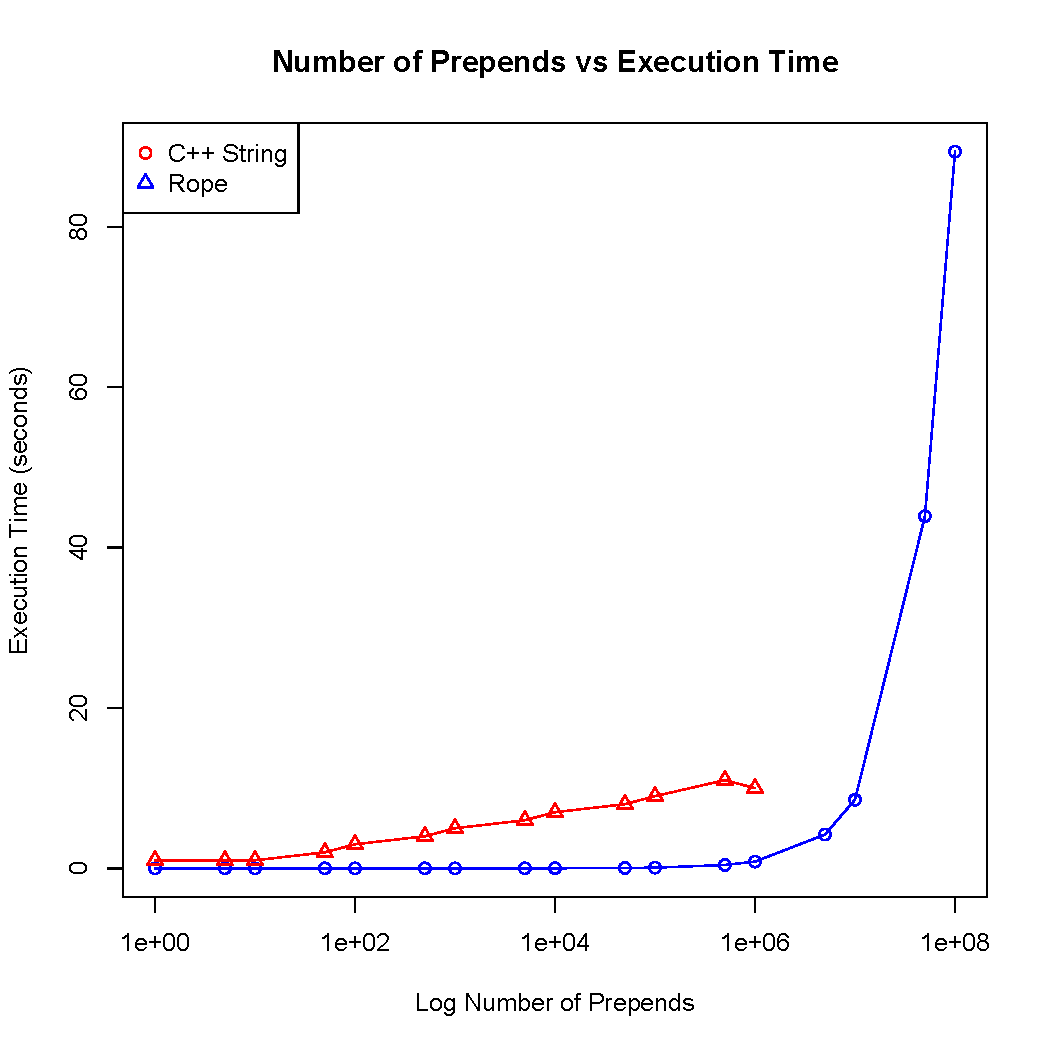
\includegraphics[scale=1.0]{prepends_vs_execution}
\caption{This graph demonstrates the running time of a benchmark that consisted of many small repeated prepend operations. We see that the rope performs significantly better than the string: the rope should support this operation very quickly, while we'd expect the C++ string to have to move everything right in order to make space at the front. Unfortunately our C++ String benchmark never terminated for the last few trials, so we have ommitted these data points. We allowed the benchmarks to run for much longer than the rope.}

\end{centering}
\end{figure}

\begin{figure}[p]
\begin{centering}
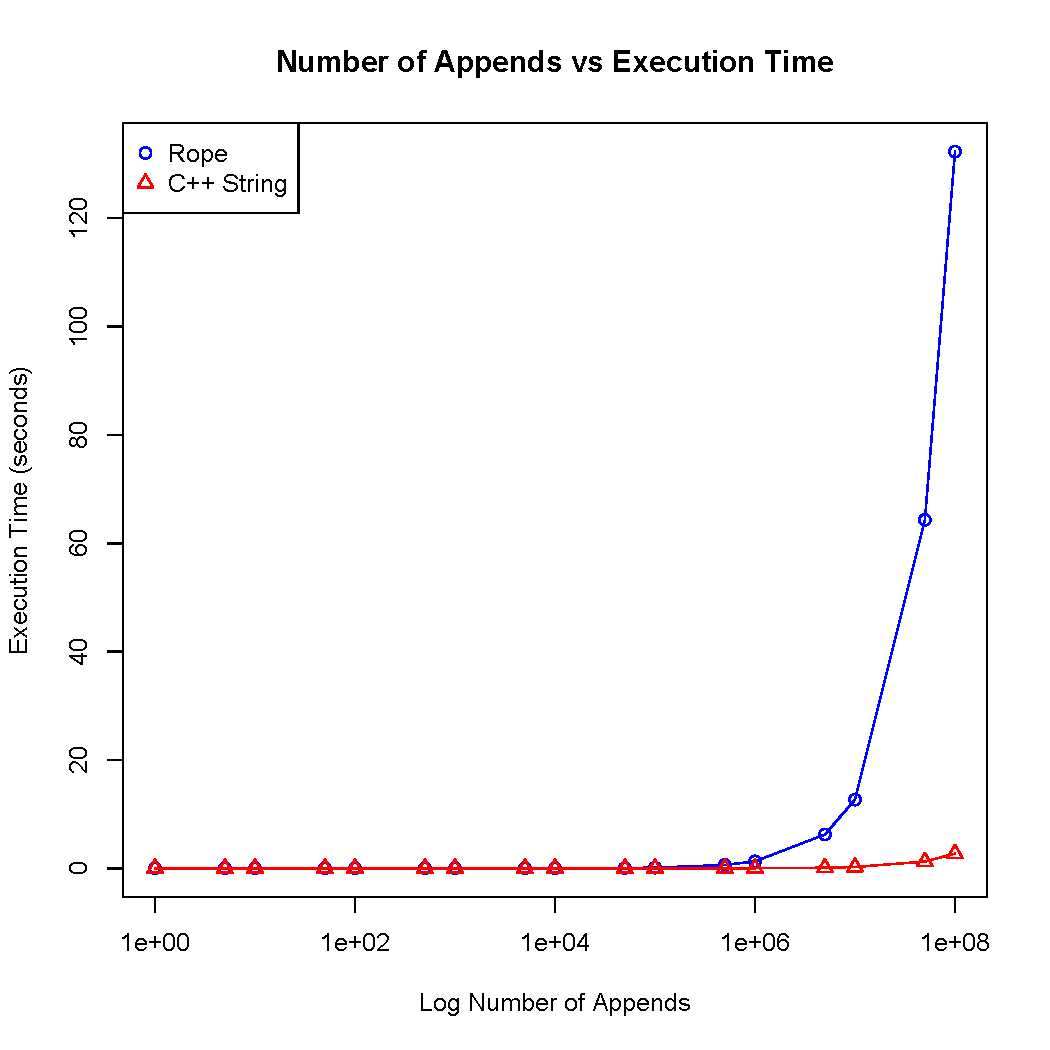
\includegraphics[scale=1.0]{append_vs_execution}
\caption{This graph demonstrates the running time of a benchmark that consisted of many small repeated append operations. Interestingly, the string performs significantly better than the rope. We suspect that the C++ implementation has optimized strings for the append operation: we suspect that we would see different behavior if string append were implemented naively. Also, we see that the rope performs approximately the same as it did for the prepend operation. This implies that it is agnostic to the end at which the string is inserted.}

\end{centering}
\end{figure}

\begin{figure}[p]
\begin{centering}
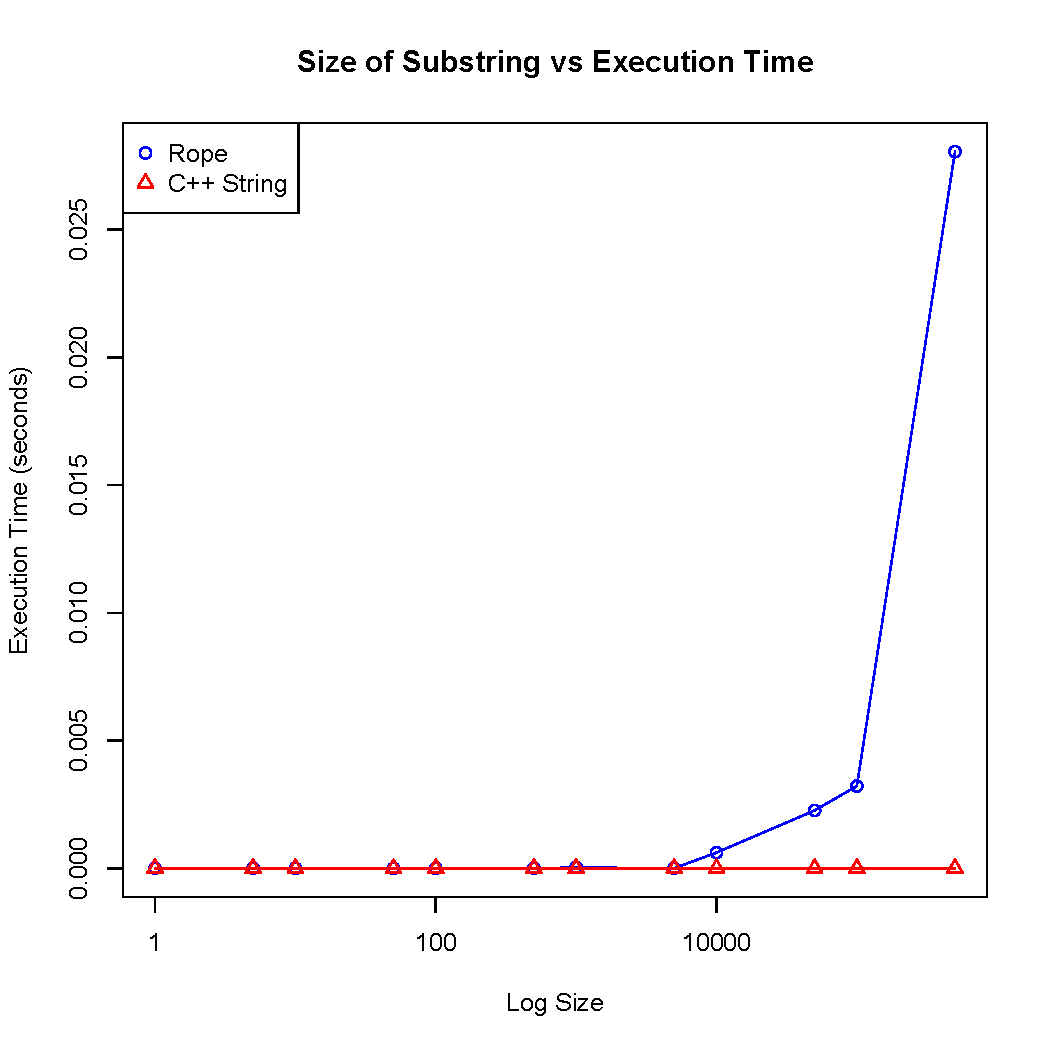
\includegraphics[scale=1.0]{substring_vs_execution}
\caption{Here we see the running time of a benchmark that consisted of extracting varying sized substrings from a large string. The string appears to dominate the substring as the size increases: the string implementation is much simpler than the rope implementation so this is not surprising.}
\end{centering}
\end{figure}

\begin{figure}[p]
\begin{centering}
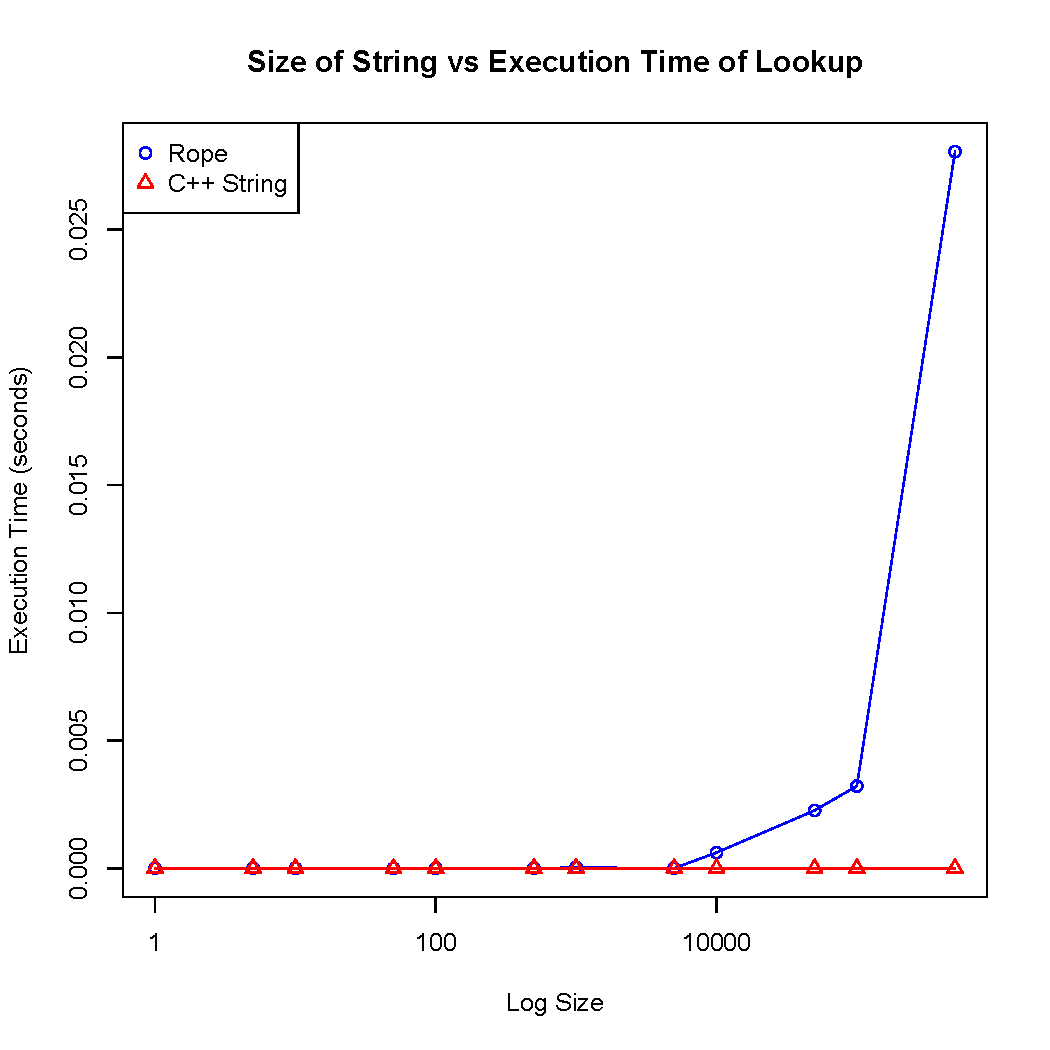
\includegraphics[scale=1.0]{size_vs_lookup}
\caption{Here we see the running time of a benchmark that consisted of lookups to random indices in a very large array. As one might guess, the string dominates the rope in this category because the array should be executing in roughly constant time, while the rope will be performing a tree traversal.}
\end{centering}
\end{figure}
\FloatBarrier
\section{Visualization}

The Rope is a somewhat complicated data structure. In order to make it easier to understand the operation of the data structure as the underlying text changes, we have implemented a simple text editor.\footnote{http://andymoreland.com/rope} This visualizer provides an input box where the user is able to perform simple text editing operations, and alongside it has a $D3$ powered visualization of the Rope's underlying data structures. An example visualization is seen in Figure \ref{editor}.

We believe that this visualization immensely clarifies how the Rope structure works: even if the formal description of the structure is unclear, a strong understanding of its operation can be obtained from the visualization very quickly.

The visualization is based off of the $C++$ rope implementation discussed in the previous section. We implement the front-end in javascript and html using $D3$, but we store the text that is input by the user by communicating over NaCl with a $C++$ program that manages a rope. Of course, it would be possible to implement the Rope in javascript itself, but we avoided doing this in an effort to avoid duplication of labor.

%% In building this simple demo, we began to consider some of the limitations of Ropes. While the immutability requirement may grant certain safety benefits, one could argue that it in a sense causes more trouble than it is worth. Consider a case where a large file has been build up via a series of sequential inserts at the end of the string. Then, when a character in the middle of the string is deleted. In the traditional implementation this first delete would require new concatenation nodes to be constructed all the way along the path from the root of the tree to node containing the edited string. Each subsequent insertion or deletion would continue to create a lot of work, including potentially memory allocations. In a text editor one often does a lot of local edits. It would be nice if a so-called `working-set' were located near the root of the tree. (We will ignore the fact that the bottleneck in most text editors these days is not the actual text manipulation but the neurons of the typist. We can still continue the exercise.)

%% One could use a splay tree for the this purpose, but then one completely forfeits some of the subtler niceties afforded by the immutability principle. For example, one could easily implmement an undo stack (very useful in a text editor!) by simply maintaining a list to previous representations of the file's string. Out of curiosity, we will forget this feature and continue to see what alterations we can apply. Suppose that in addition to having a completely mutable tree, we also had mutable string buffers. Then a series of local edits would splay a node up to the root, and as long as the buffer was moderately full every insert/delete would only take time proportional to the size of the buffer. This unfortunate fact means that this approach is unlikely to lead to any asymptotically better algorithms. We can see this by assuming that we have a block size of $b$. Though this hasn't been mentioned, supose we could somehow force each buffer to be at least half full. This would guarantee $\Theta(n/b)$ nodes in our tree, so splaying would take $O(\log n/b)$, but every individual operation at a node would also take $O(b)$ for a total time of $O(\log n/b) + O(b) = O(\log n) - O(\log b) + O(b) = O(\log n) + O(\log )$, which is nothing special. As long as $b$ on the order of $\log n$, then we won't lose any ground. Perhaps such a structure would be faster in practice due to the fewer allocations. As mentioned, insertions and deletions from the middle could force $O(\log n)$ new nodes per operation in the immutable rope, where as in this its $O(1 / \log n)$ allocations per insertion or deletion because you only would need a new node wheneve you add $\log n$ new characters! This is certainly better and likely indicates significant performace benefits.

\begin{figure}[t]
\begin{centering}
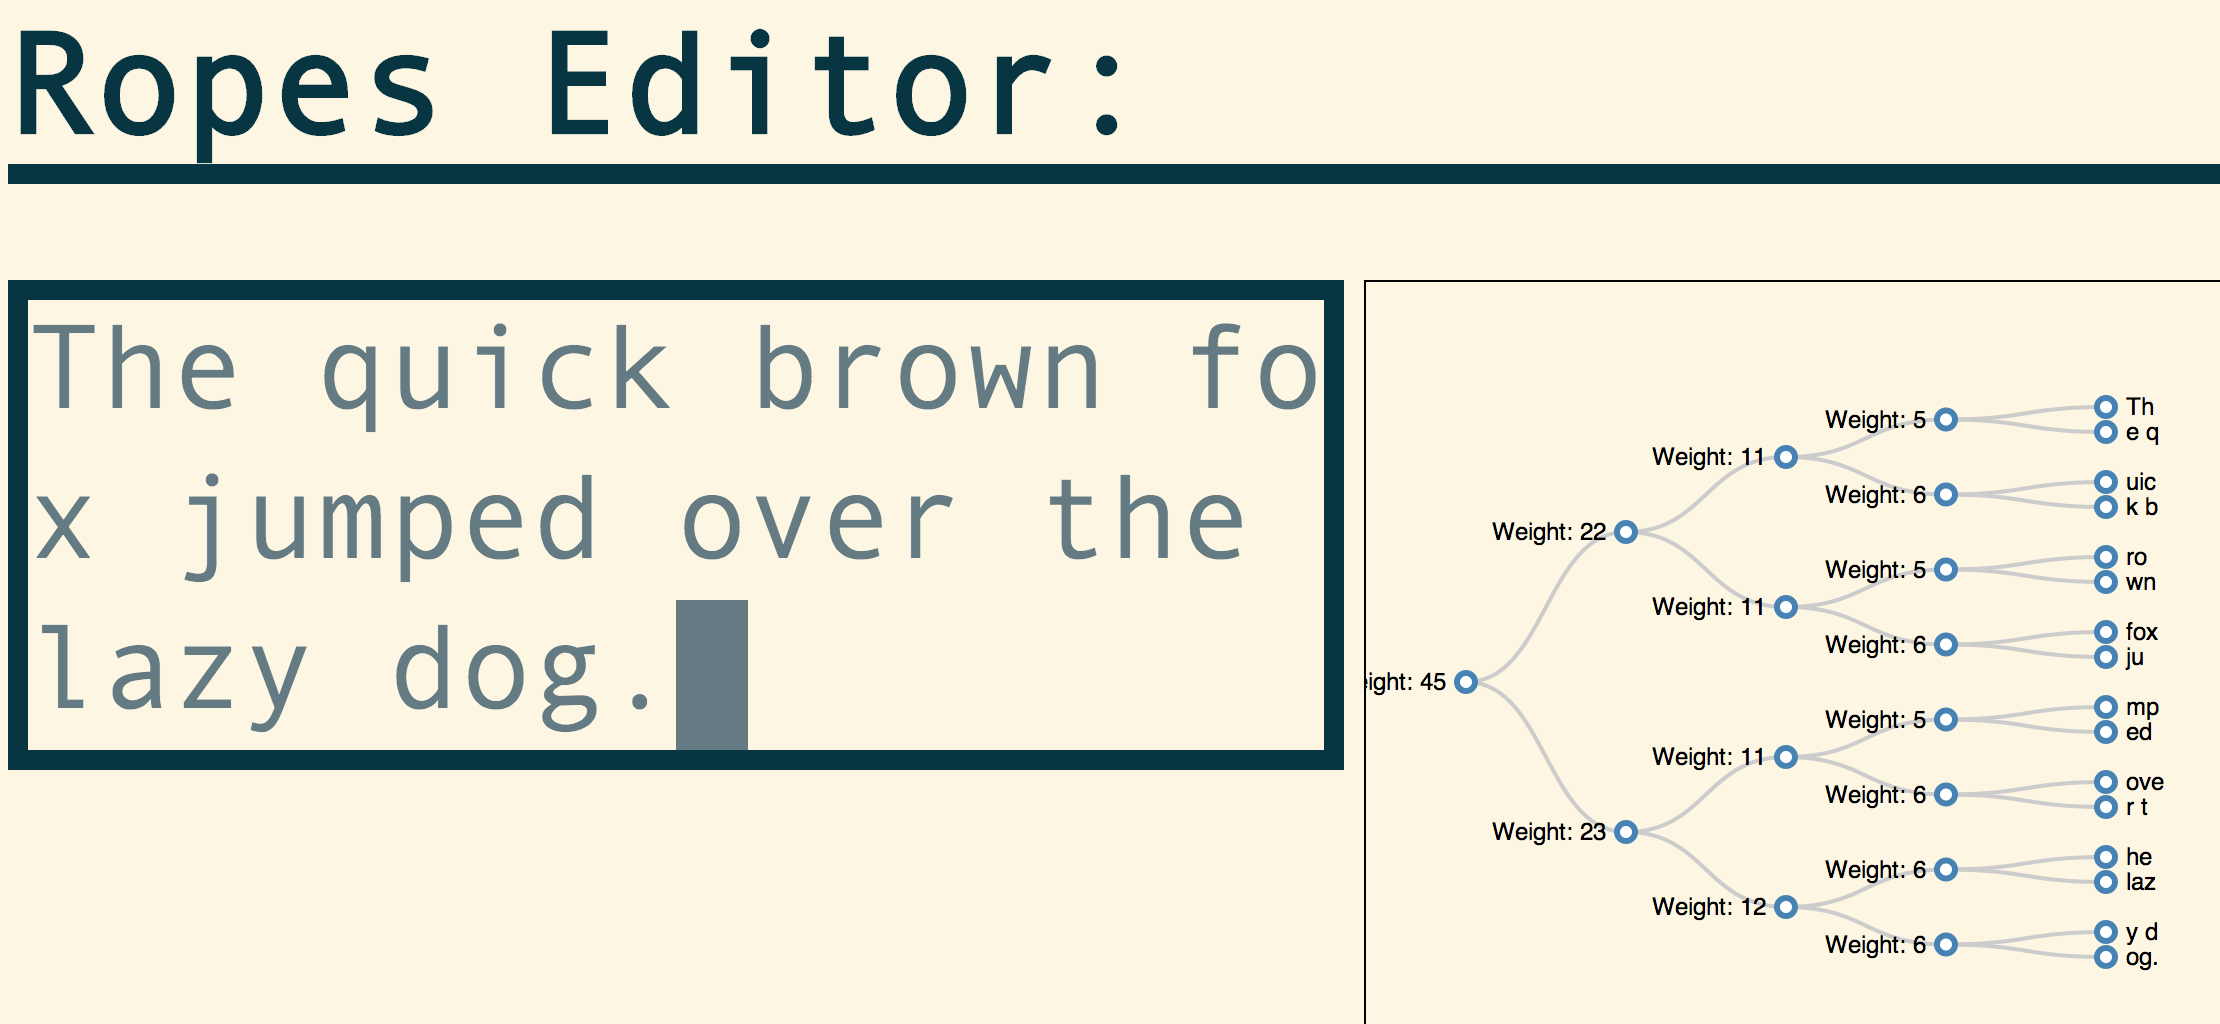
\includegraphics[scale=0.35]{editorImage1}
\caption{This figure demonstrates the visualization that we implemented in order to display a Rope's internal structure. On the left the user is able to enter a string and on the right we see the state of the Rope's internals after adjustment.}\label{editor}

\end{centering}
\end{figure}

\section{Conclusion}

In this paper we have presented the Rope datastructure as described by Hans-J. Boehm, Russ Atkinson and Michael Plass in 1995. It is an efficient datastructure for immutable operations on large strings. We have demonstrated the core operations and algorithms for this datastructure and shown that they operate efficiently.

In addition, we have contributed a novel implementation of the Rope datastructure based on a splay tree representation. We provide benchmarks that show that the datastructure performs roughly as expected in several standard scenarios.

Finally, we have presented our visualization of the rope data structure. We implemented a browser-based visualizer that interacts over NaCl with a Rope in order to power a simple text editor. While the editor is in action, we display the internal tree structure of the rope alongside the user's input area. 


\end{document}
